\documentclass[12pt,fleqn]{article}
\usepackage{a4wide}
\usepackage{ngerman}
%\usepackage{umlaut}
%\usepackage[dvips]{graphicx}
\usepackage[utf8]{inputenc}
\usepackage[]{listings}
\lstset{literate=%
    {Ö}{{\"O}}1
    {Ä}{{\"A}}1
    {Ü}{{\"U}}1
    {ß}{{\ss}}1
    {ü}{{\"u}}1
    {ä}{{\"a}}1
    {ö}{{\"o}}1
    {~}{{\textasciitilde}}1
}
% \usepackage[latin1]{inputenc}
\usepackage{amsmath}
\usepackage{amssymb}

\usepackage{bm}
\usepackage[pdftex]{graphicx}
\DeclareGraphicsExtensions{.ps.gzbody,.ps, .eps.gzbody, .eps}
\DeclareGraphicsRule{.ps.gzbody}{eps}{.ps.gzheader}{`gzcat #1}
\DeclareGraphicsRule{.eps.gzbody}{eps}{.eps.gzheader}{`gzcat #1}
\usepackage{color}

\usepackage{vmargin}
\setpapersize{A4}
\setmarginsrb{2.0cm}{1.5cm}{2.5cm}{2cm}{1.2\baselineskip}{1cm}{1.2\baselineskip}{0cm}
\newcommand{\mpraktikum}{\textbf{MT Praktikum - Word Embeddings \& NNLM} } 

\newcommand{\mhead}{\pagestyle{myheadings}
        \markright{\underline{\textsf{\mpraktikum - \today  -  \hfill Eunah Cho, KIT, eunah.cho@kit.edu}}}}

\newcommand{\mlogo}{ \sffamily \vspace*{-10mm}
  \begin{minipage}{2cm}
    
\includegraphics[scale=0.3]{Bilder/KIT.jpg}
  \end{minipage}
  \hfill
  \begin{minipage}{10.5cm}
    \textsf{\large{Karlsruhe Institute of Technology}} \\[0.2ex]
    \textsf{\large{Dr. Eunah Cho}}\\  
    \textsf{\large{Institute for Anthropomatics and Robotics, Interactive Systems Labs}}\\[0.2ex]  
    \textsf{eunah.cho@kit.edu} 
  \end{minipage}
  \rmfamily
  \vspace*{2cm}

   \centerline{\Large \mpraktikum } 
   \vspace{1ex}
   \centerline{\Large \today}
  } 
\setlength{\parindent}{0cm}
\setlength{\unitlength}{1cm}  
\addtolength{\marginparsep}{3mm}
\sloppy 

\begin{document}
\thispagestyle{empty}


\mhead

\mlogo

\vspace{2cm} 
%%%%%%%%%%%%%%%%%%%%%%%%%%%%%%%%%%%%%%%%%%%%%%%%%%%%%%%%%%%%%%%%%%%%%%
% \loes \medskip \\   % Signalverarbeitung
%%%%%%%%%%%%%%%%%%%%%%%%%%%%%%%%%%%%%%%%%%%%%%%%%%%%%%%%%%%%%%%%%%%%%%

Um die Aufgaben auszuführen, können Sie Ihre Daten in folgendem Verzeichnis speichern: 
\texttt{/project/smtstud/ss17/systems/USERNAME/} 

\vspace{0.5cm} 
We are going to use a pre-trained word vectors. Copy this word vector file into your directory. 

\vspace{0.5cm}
\texttt{/project/smtstud/ss17/data/vec/Wemb.en.filtered.lowered} 

\vspace{0.5cm} 
Later you are going to calculate the cosine similarity of words represented in vector space. Copy the script into your directory. 

\vspace{0.5cm} 
\texttt{/project/smtstud/ss17/bin/vector.py} \\

\vspace{0.5cm} 
\textbf{A. Word Embeddings} \\ 

\begin{enumerate}



\item In the last page, you can find visualization from word embeddings obtained from English and French machine translation data. It is also available at http://i13pc106.ira.uka.de/$\sim$echo/research.pdf. 
Words are filtered under the topic ``Research''. \\ 

\begin{itemize} 
 \item Find at least three groups where you can see the similarity in meanings and mark on the visualization. You can also check a English-French dictionary: http://enfr.dict.cc/. 
\end{itemize}

% \textit{Q. Can you spot similarities between English and French words? Find at least three groups where you can see the similarity in meanings and mark on the visualization.} \\ 
% 
% Following table gives you a brief information on words in French and their meaning in English. You can also check a English-French dictionary: http://enfr.dict.cc/.  \\ 
% 
% \begin{table}[h] 
%  \begin{center} 
%   \begin{tabular}{l|l}
%    French word & Meaning in English \\  \hline 
% clinique & clinical \\ 
% scientifique & scientific \\ 
%    scolaire & school \\ 
%    travail & job, work \\ 
%    chercheur & researcher \\ 
%   \end{tabular}
%  \end{center}
% \end{table}



\item We are going to examine pre-trained 200-dimensional vectors for 10K English vocabulary.  
% \texttt{head -n 2 Wemb.en.filtered.lowered | tail -n 1 } \\ \\ 
Examine the format of the file.  
% It consists of a word and its vector representation in a 200-dimensional space. \\ 

Word vectors represent semantic and syntactic relationship between words. For example, \textit{lady} should be closely related with \textit{woman}. Check their vector values. 

\begin{itemize} 
 \item Check vector values of the word \textit{lady} and \textit{woman}. 
\end{itemize}


\begin{table}[h] 
 \begin{center} 
  \begin{tabular}{l|p{2cm}|p{2cm}|p{2cm}|p{2cm}|l|p{2cm}}
   word & $v_0$ & $v_1$ & $v_2$ & $v_3$ & ... & $v_{199}$ \\  \hline 
lady & & & & ... & \\ 
woman & & & & ... & \\ 
  \end{tabular}
 \end{center}
\end{table}

%We can check the vector values of the two words. \\ 
% 
% \texttt{lady: 0.01361018 0.04732877 -0.00540839 -0.09349286 ..... -0.05747397 0.01850754} \\ 
% \texttt{woman: 0.07737311 0.04137088 -0.01775537 -0.13916844 ..... -0.02483073 -0.02679169} \\ 

% As you can see, it is hard for us to understand the vector representation as it is. Therefore, we are going to calculate their distance using a script. 

\item We can check the similarity of the words by loading the vectors and calculating the distance between them. \\ 

% \texttt{cp ../scripts/vector.py . } \\ 
\texttt{python vector.py} \\ 

\begin{itemize} 
 \item What is the most similar word to the word \textit{lady}? What is their similarity? 
 \item Find the most similar word for following words and fill the table. 
 \begin{table}[h] 
  \begin{center} 
     \begin{tabular}{c|c|c}
      Input word & Most similar word & Similarity \\  \hline 
      lady & & \\ 
      book & & \\ 
      mother & & \\ 
      school & & \\ 
      great & & \\ 
      tree & & \\ 
     \end{tabular}
  \end{center}
\end{table}
\item Find the similarity score of following words and fill the table. When is the similarity score high? 
\begin{table}[h] 
   \begin{center} 
         \begin{tabular}{c|c|c}
          word A & word B & similarity \\  \hline 
          father & dad &  \\ 
          human & animal &  \\ 
          apple & big & \\ 
          soccer & football & \\ 
         \end{tabular}
   \end{center}
\end{table}

\item Find the word which fits in the semantic relationship.

\begin{table}[h] 
   \begin{center} 
         \begin{tabular}{lc}
man : husband = woman :& wife \\ 
grass : green = sky : & \\ 
tree : forest = water : & \\ 
         \end{tabular}
   \end{center}
\end{table}
\end{itemize}
\end{enumerate}  
% 
% \item There are three options. \\ 
% \begin{figure} [h] 
% \hspace{1.5cm} 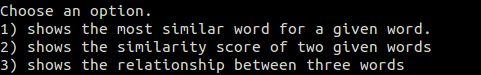
\includegraphics[width=10cm]{options.png} 
% \end{figure}
% \\ 
% By choosing 1, we can find the most closely mapped word for a given word. Type 1, and find the most closely located word for following words. For example, we can find the most similar word to \textit{lady} as follows. \\ 
% \begin{figure} [h] 
% \hspace{1.5cm} 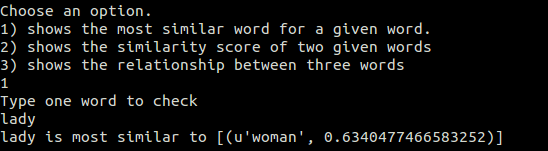
\includegraphics[width=11cm]{lady.png} 
% \end{figure}
% \\ 
% \textit{lady} is most similar to \textit{woman} according to the word vectors. Their similarity is 0.63. \\ \\ 
% \textit{Q. Find the most similar word for following words and fill the table.} \\ 
% 
% \begin{table}[h] 
%   \begin{center} 
%      \begin{tabular}{c|c|c}
%       Input word & Most similar word & Similarity \\  \hline 
%       lady & woman & 0.63\\ 
%       book & & \\ 
%       mother & & \\ 
%       school & & \\ 
%       great & & \\ 
%       tree & & \\ 
%      \end{tabular}
%   \end{center}
% \end{table}
% \newpage
% \item You can also calculate the similarity between two words by choosing option 2. Following example shows how to get similarity score for two words. 
% \\ 
% \begin{figure} [ht] 
% \hspace{1.5cm} 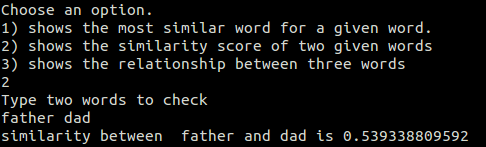
\includegraphics[width=11cm]{similarity.png} 
% \end{figure}
% \\ 
% 
% \textit{Q. Find the similarity score of following words and fill the table. When is the similarity score high? } \\ 
% \begin{table}[ht] 
%    \begin{center} 
%          \begin{tabular}{c|c|c}
%           word A & word B & similarity \\  \hline 
%           father & dad & 0.54 \\ 
%           human & animal &  \\ 
%           apple & big & \\ 
%           soccer & football & \\ 
%          \end{tabular}
%    \end{center}
% \end{table}
% \item Finally, you can tell the relationship between words. 
% \\ 
% \begin{figure} [h] 
% \hspace{1.5cm} 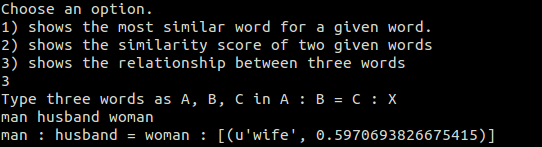
\includegraphics[width=11cm]{relationship.png} 
% \end{figure}
% \\ 
% Thus, the relationship between words \textit{man} and \textit{husband} is similar to the relationship between words \textit{woman} and \textit{wife}. From the same way, we can explore semantic closeness and relationships captured in the word vectors. \\
% \\ 
% \newpage
% \textit{Q. Find the word which fits in the semantic relationship.} \\ 
% 
% \begin{table}[ht] 
%    \begin{center} 
%          \begin{tabular}{lc}
% man : husband = woman :& wife \\ 
% grass : green = sky : & \\ 
% tree : forest = water : & \\ 
%          \end{tabular}
%    \end{center}
% \end{table}
% \item Word vectors can also tell a concept which does not fit into the general topic. 
% \begin{figure} [h] 
% \hspace{1.5cm} 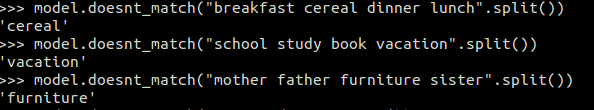
\includegraphics[width=12cm]{doesntmatch.png} 
% \end{figure}
% \\ 
% For example, \textit{cereal} does not fit with other words indicating meals of the day (\textit{breakfast, lunch, dinner}). When talking about studying (\textit{school, study, book}), \textit{vacation} is a distanced topic. Also, \textit{furniture} does not fit into a family member description (\textit{mother, father, sister}). \\
% % \item You can also try with other words! 




\newpage 

\vspace{0.5cm} 
\textbf{B. Neural Language Model} \\ 

\begin{enumerate} 

\item Take a look into the log file of training a neural language model. \\ 
\texttt{/project/smtstud/ss17/data/rnnlm/Train.log} \\ 

\begin{itemize} 
 \item How is the perplexity score for development data? 
\end{itemize}



\item There are four RNN language models trained. You can find them in \\ 
\texttt{/project/smtstud/ss17/models/rnnlms/} 

All models are trained with top 5,000 words. 
\begin{enumerate} 
 \item Forward LM, two layers 
 \item Backward LM, two layers 
 \item Forward LM, two layers but half of the size  
 \item Forward LM, one layer 
\end{enumerate}

We are going to apply each LM on the test data. 

\texttt{/project/smtstud/ss17/data/rnnlm/test.de} \\ 

\begin{itemize} 
 \item Which sentences in the test data should have lower perplexity? Why? 
\end{itemize}

\newpage 

\item Copy the following script into your directory and run it in your directory. 

\texttt{/project/smtstud/ss17/bin/rnnlm/Test.back\_forward.sh} 

The script calculates perplexity for each sentence using the backward and the forward LM. 

\begin{itemize} 
 \item How is the perplexity for each sentence using each model? 
\end{itemize}


\begin{table}[ht] 
   \begin{center} 
         \begin{tabular}{|p{12cm}|p{1.5cm}|p{1.8cm}|} \hline 
& Forward & Backward \\  \hline 
ich melde mich f\"{u}r die Konferenz an . &  & \\ \hline
ich melde mich f\"{u}r die Konferenz auf . &  & \\  \hline \hline
ich schlage mit der rechten Hand auf . & & \\ \hline
ich schlage mit der rechten Hand vor . & & \\ \hline \hline
mein Freund , den ich seit vielen Jahren kenne , ist nach Stuttgart gezogen . & & \\ \hline
mein Freund , den ich seit vielen Jahren kenne , sind nach Stuttgart gezogen . & & \\ \hline \hline
die Verkäuferin ist nett . & & \\ \hline
die Marklerin ist nett . & & \\ \hline 
         \end{tabular}
   \end{center}
\end{table}

\item For the same test data, try an LM that has half-sized dimensions and another LM that has only one layer. Copy the following script into your directory and run it in your directory.

\texttt{/project/smtstud/ss17/bin/rnnlm/Test.halfdim\_onelayer.sh} 

\begin{itemize} 
 \item How is the perplexity for each sentence using each model? 
\end{itemize}

\begin{table}[ht] 
   \begin{center} 
         \begin{tabular}{|p{12cm}|p{1.5cm}|p{1.8cm}|} \hline 
& HalfDim & OneLayer \\  \hline 
ich melde mich f\"{u}r die Konferenz an . &  & \\ \hline
ich melde mich f\"{u}r die Konferenz auf . &  & \\  \hline \hline
ich schlage mit der rechten Hand auf . & & \\ \hline
ich schlage mit der rechten Hand vor . & & \\ \hline \hline
mein Freund , den ich seit vielen Jahren kenne , ist nach Stuttgart gezogen . & & \\ \hline
mein Freund , den ich seit vielen Jahren kenne , sind nach Stuttgart gezogen . & & \\ \hline \hline
die Verkäuferin ist nett . & & \\ \hline
die Marklerin ist nett . & & \\ \hline 
         \end{tabular}
   \end{center}
\end{table}

\item Feel free to try your own examples by inputting your own \texttt{testdata} in the bash file. 

\newpage
\begin{figure}[ht]
\vspace{-3cm} 
 \hspace{-1cm} 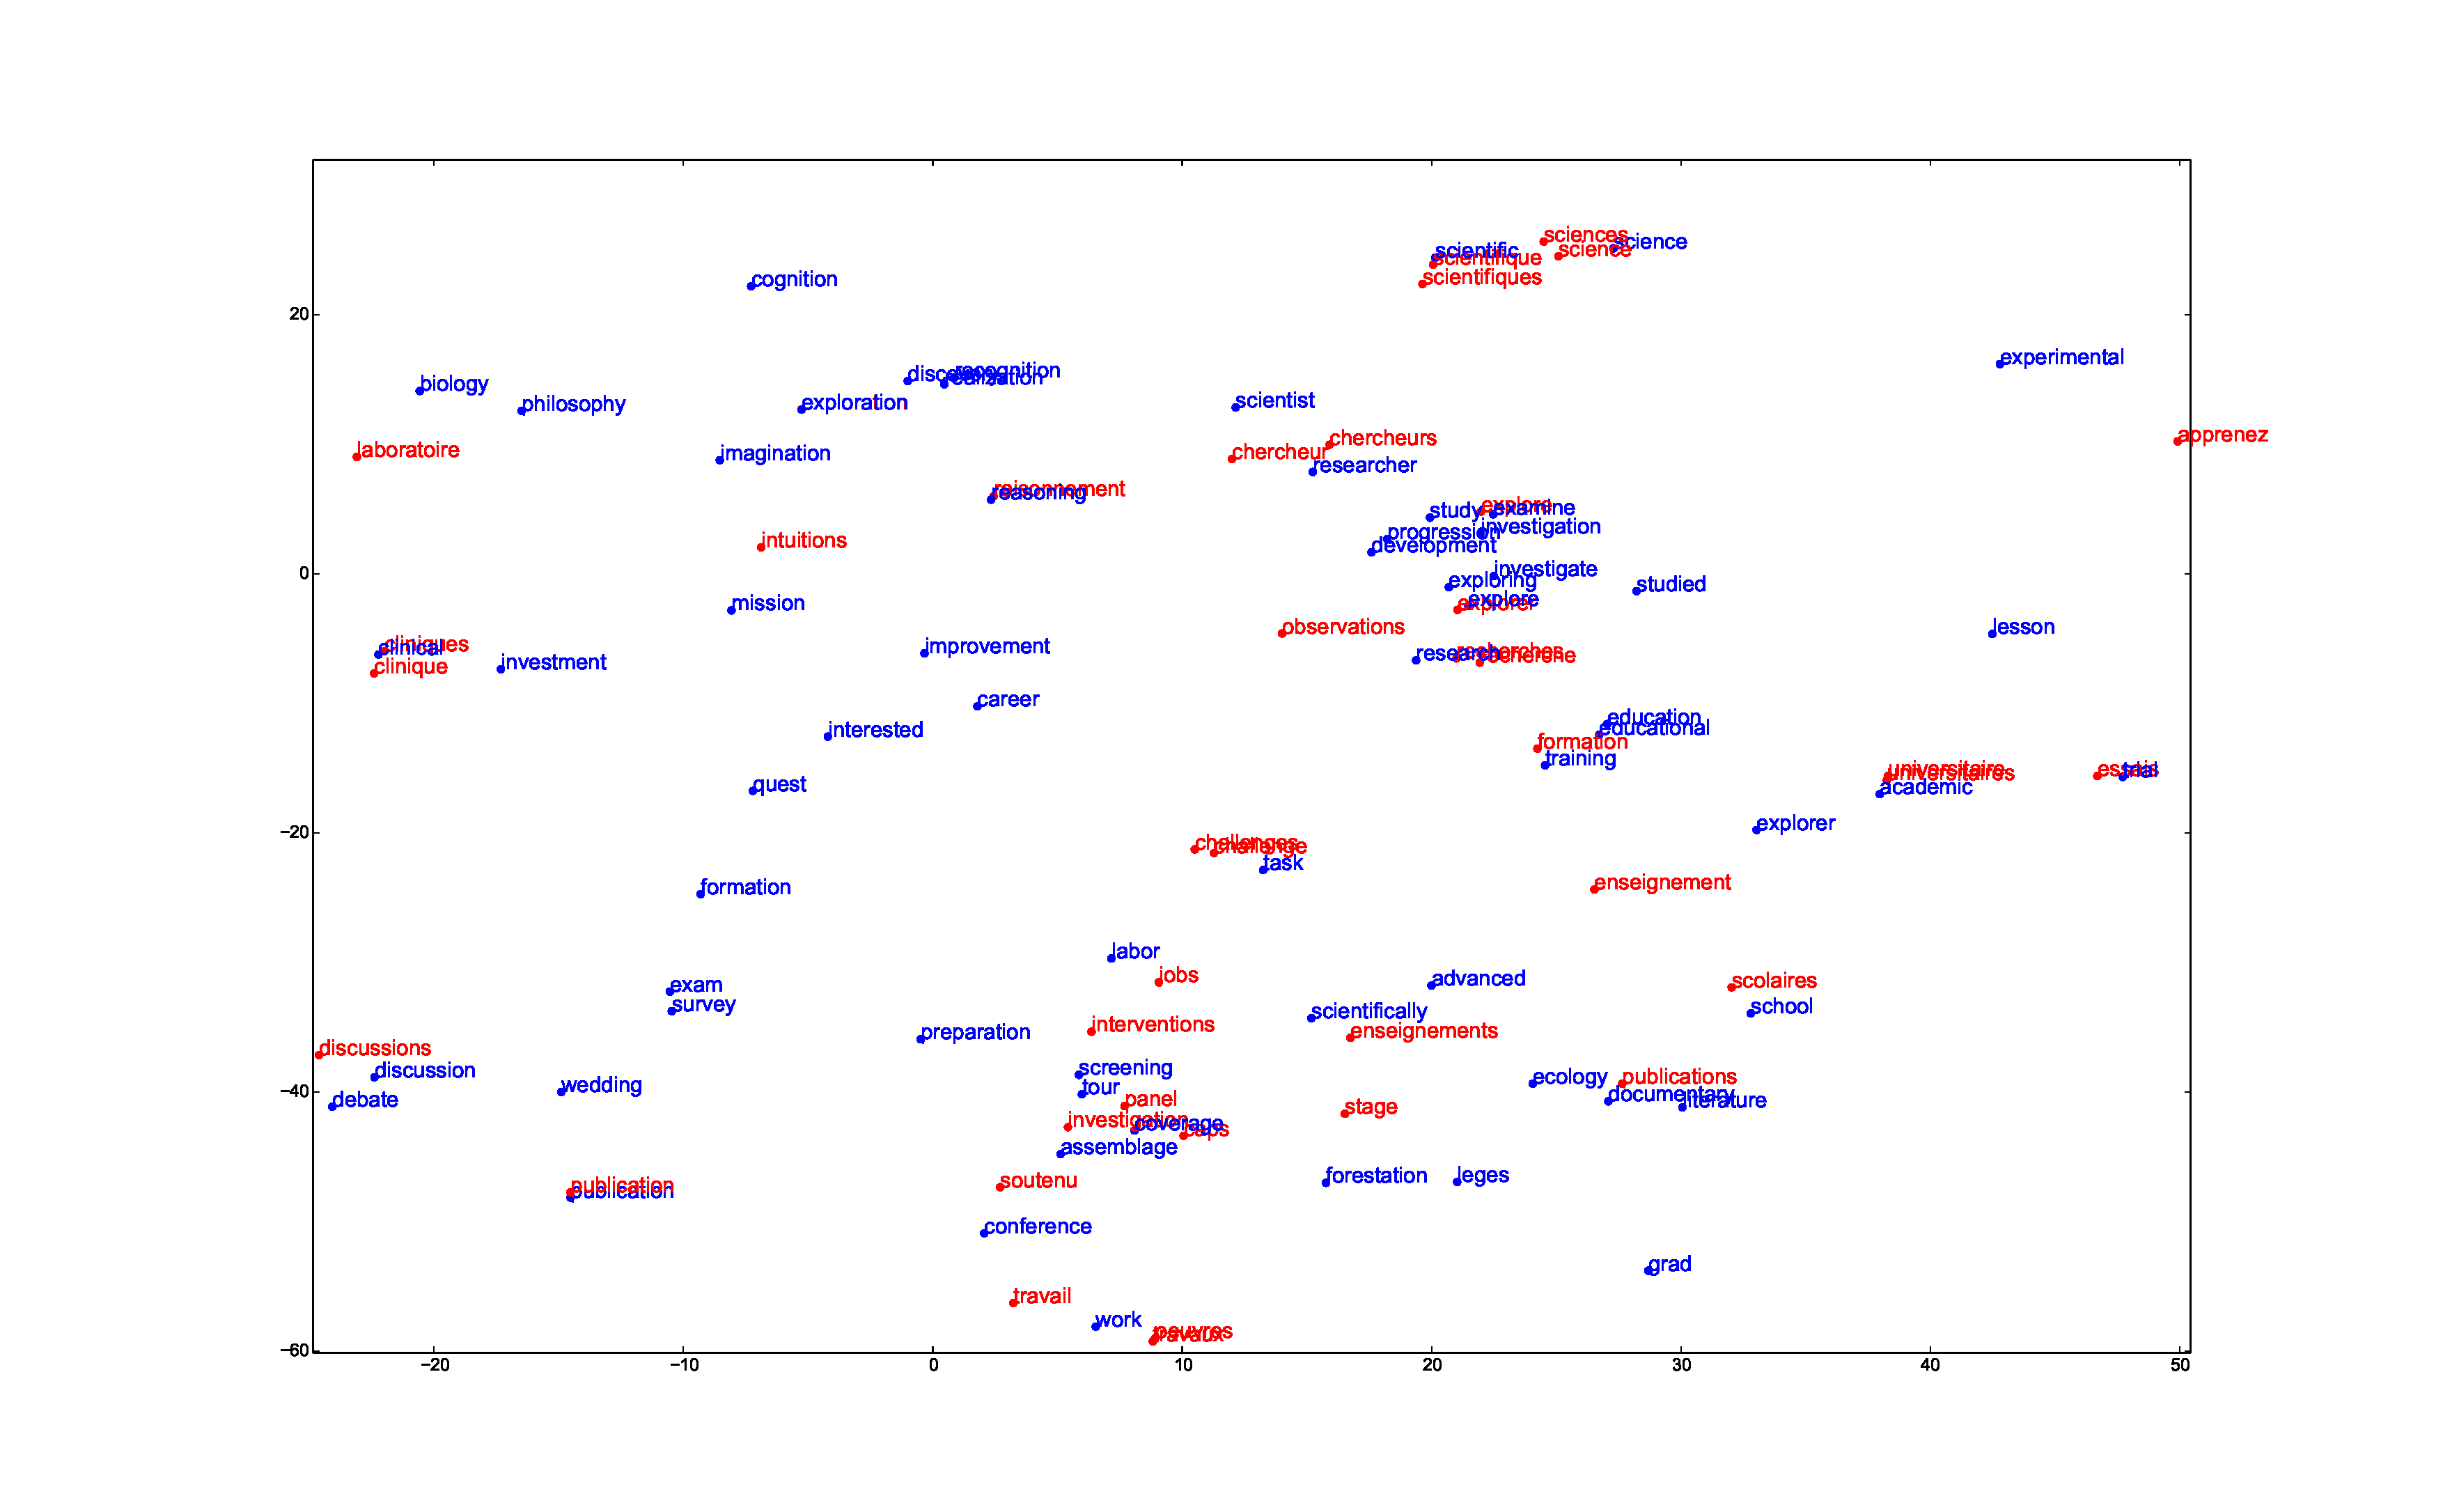
\includegraphics[angle=90, width=19cm]{research.eps} 
\end{figure}

\newpage 



\end{enumerate}




%%%%%%%%%%%%%%%%%%%%%%%%%%%%%%%%%%%%%%%%%%%%%%%%%%%%%%%%%%%%%%%%%%%%%%%%%%%%%%%%%%%%%%%%%%%%%%%%%%%%%%%%%%%%%%%%
\end{document}

